\documentclass{article}

\usepackage{fancyhdr}
\usepackage{ragged2e}
\usepackage{graphicx}
\usepackage{caption}
\usepackage{geometry}
\usepackage{amsmath}
\usepackage{rotating}

\usepackage{listings}
\usepackage{color}

\definecolor{dkgreen}{rgb}{0,0.6,0}
\definecolor{gray}{rgb}{0.5,0.5,0.5}
\definecolor{mauve}{rgb}{0.58,0,0.82}

\lstset{frame=tb,
  language=Java,
  aboveskip=3mm,
  belowskip=3mm,
  showstringspaces=false,
  columns=flexible,
  basicstyle={\small\ttfamily},
  numbers=none,
  numberstyle=\tiny\color{gray},
  keywordstyle=\color{blue},
  commentstyle=\color{dkgreen},
  stringstyle=\color{mauve},
  breaklines=true,
  breakatwhitespace=true,
  tabsize=4
}

\setcounter{secnumdepth}{1}

\usepackage{chngcntr}
\counterwithin{figure}{section}

\renewcommand*{\thepage}{C\arabic{page}}

\pagestyle{fancy}
\lhead{ACME Robotics}
\chead{\#8367}
\rhead{\ifcontents Contents \else Week \thesection \fi}

\newif\ifcontents
\contentstrue

\makeatletter
\renewcommand{\@seccntformat}[1]{}
\makeatother

\begin{document}\contentsfalse
\subsection{Sorter CAD}
%! CAD the sorter.
Ashlin and Aidan continued to finalize the sorting system for the robot and completed the CAD model of the sorter. Aidan realized a flaw with the system, if a ball then a cube went into the sorter right after each other then the cube could jam the sorter. This was because the interior length of the rotating piece was almost 4 inches long, so if a ball then a cube went in the sensor would read the ball and then start rotate but the cube would block the rotating and jam the servo. Kelly, Ashlin, Aidan, and Jon all thought of ideas to solve this problem including shortening the sorter's dimensions, creating a servo powered gate, or just changing the whole system. The team finally decided to solve the problem once the sorter was fabricated. The problem could only occur if the two items went into the sorter immediately after each other. The team believed that the intake would probably space out the items sufficiently so this problem wouldn't occur, and if it did occur small adjustments could be made to increase the space between items.

\subsection{Develop X-rail based lift}
%! Develop a CAD model of the x-rail based lift.
 After downloading all the required parts from Actobotics website and importing them into Inventor. He began assembling them per the design previously created. The first issue that had to be resolved was the mounting of the bearing bracket onto the x-rail. Because the maximum amount of space should be left on the inside of the lift, a mounting scheme other than the one suggested by Actobotics would have to be used. By swapping out the standoffs that came with the kit for shorter ones, the bearings could be brought closer to the x-rail they were attached to, reducing the spacing between stages to about a quarter inch. This reduced clearance between the stages necessitated another change. The default mounting hardware would fit, but as soon as bolts were added to the model the bolts would collide with the opposite rail. To resolve this, separate mounting hardware had to be found on the Actobotics website, allowing the bolts to clear each other. It would still be neccecary to use lower profile 6-32 bolts than the standard Tetrix ones, but they should be able to be found at a hardware store. The inner carriage turned out to a be a little different than planned. There was no way to run more bearings along the front and back of the first stage box, because those grooves were already occupied by the bearings fixed to the top of the fixed stage. This meant that for the second stage to mount, a second piece of x-rail would have to be attached to the inside of the first piece, allowing the carriage to attach to it, or the carriage would have to run along the inside of the first stage. This would be possible with x-rail, because if the bearings pressed against the inside, the v-groves would prevent it from rotating forward and back, provided the top and bottom sets of bearings were spaced far enough apart to reduce the force applied laterally. This, however, would necessitate a different mounting strategy, because the brackets would have to attach to the end of the x-rail, rather than the sides. Unfortunately, the hole pattern on the end of the x-rail did not nicely match up with the hole pattern on the bracket, so Kelly decided to put two smaller vertical pieces of x-rail on either side of the cross-brace that would support the scoring mechanism, and then mount the bearings to that. 

\subsection{CAD Lander Clamp}
%! Create a latch in CAD that will be used to attach to the lander. 
To lower and raise the robot from the lander, the team decided to attach a latch to their lift. The team decided to do this because by attaching it to the scoring lift the team would not have to create a separate lift or arm to hang from. Kelly made the original prototype for this mechanism - which used two pillow blocks that when placed around the hook on the lander had a bar slid through to have the robot hang. Jon then used this basic prototype to CAD a more finalized design.

\begin{figure}
    \centering
    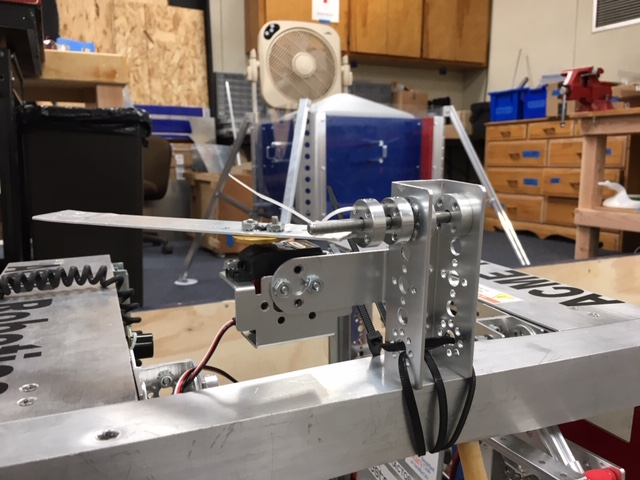
\includegraphics[width=.6 \textwidth]{06_10-08/images/latch1.JPG}
    \caption{Latch Prototype}
    \label{fig: Latch CAD1}
\end{figure}

\begin{figure}
    \centering
    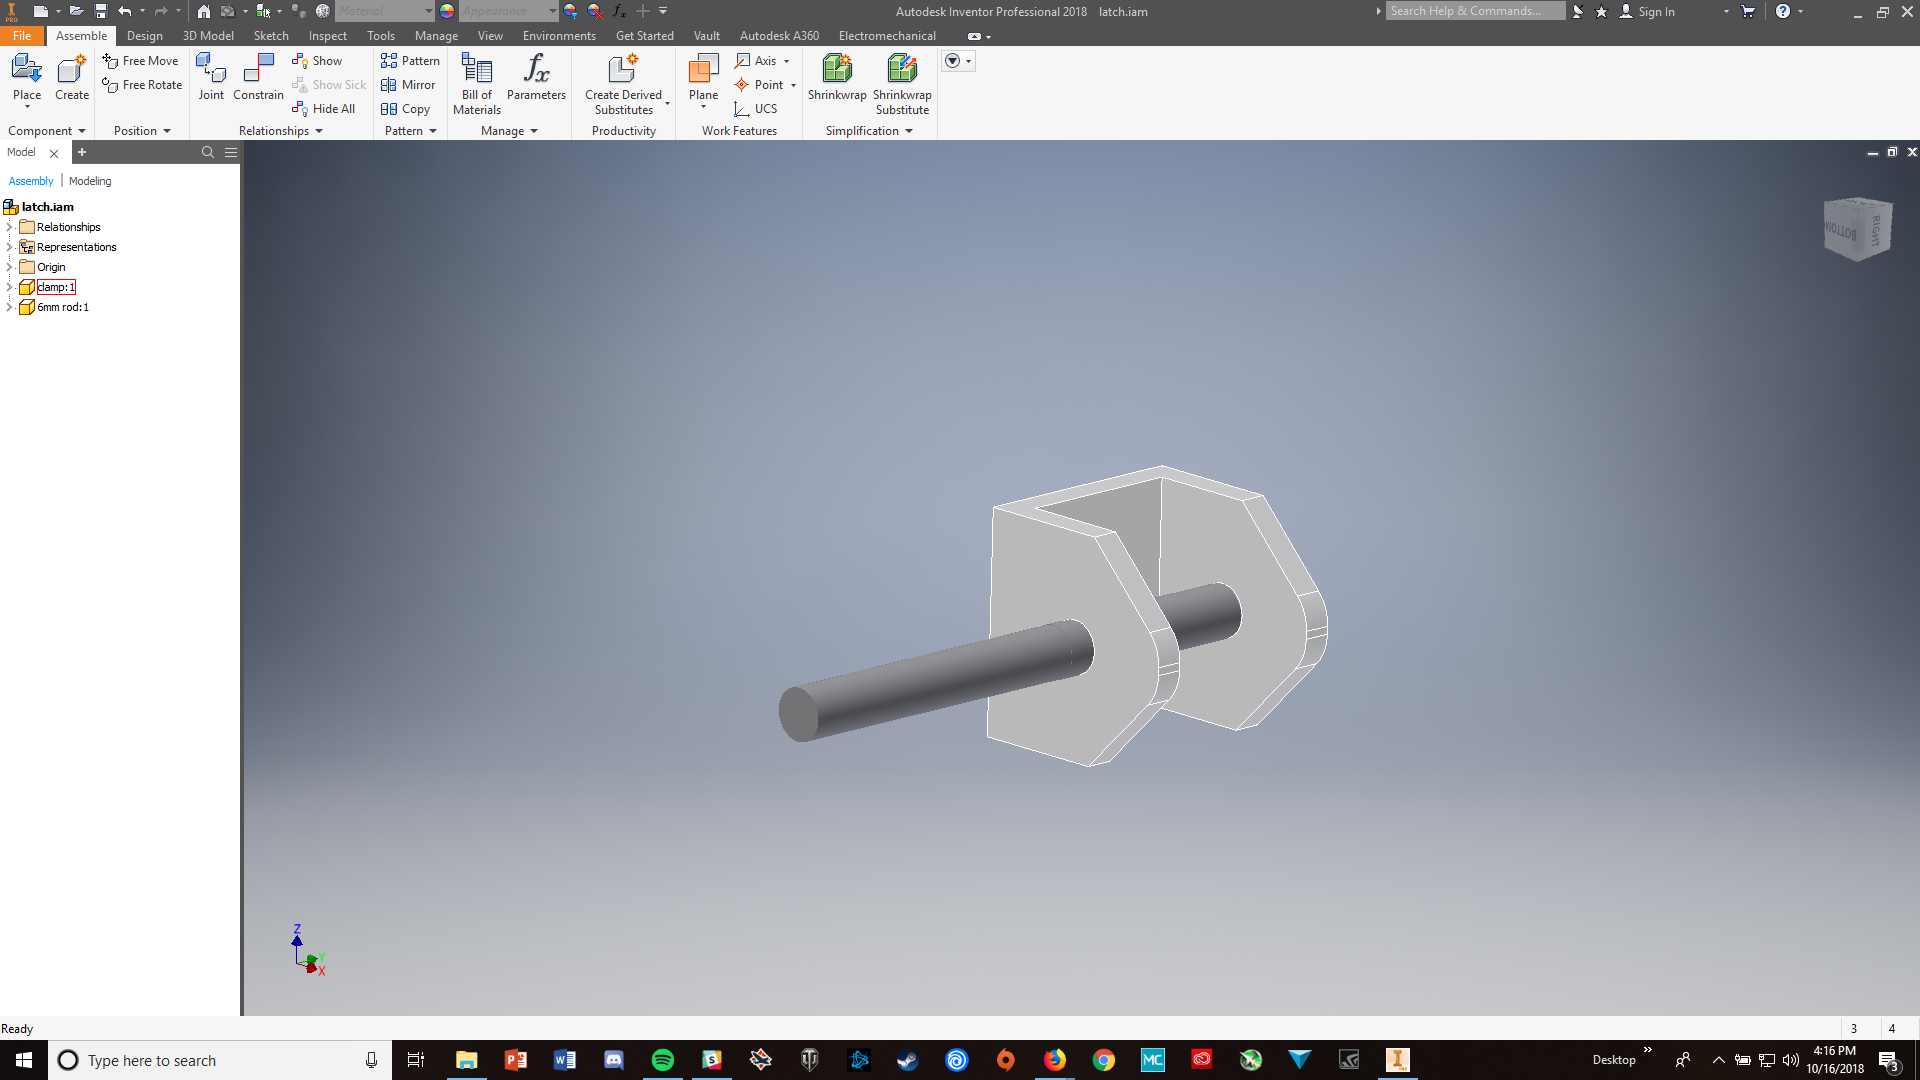
\includegraphics[width=.6 \textwidth]{06_10-08/images/latch.png}
    \caption{Latch CAD}
    \label{fig: Latch CAD2}
\end{figure}

\subsection{Finalize robot design}
%! Discuss the final robot design with the team.
The team got together and went over the robot design, making sure that everything had been considered and accounted for before the final stages of CAD were completed and parts were ordered. Everybody presented prototypes and CAD that they had been working on, and the team decided whether or not to stick with it, and discussed any problems that might arise as the parts went into production. The first thing to decide was the type of drive base. The team had used mecanum drives the previous two years, and was confident they could build it correctly, but did not want to dismiss a tank drive. The tank drive that was being considered was a chain driven 6-wheel drop center west coast drive. The mecanum drive being considered was the same thing that the team had used to success last year, a belt-driven mecanum drive, with dead axles constrained between drive plates giving it extra rigidity. Oren had made some improvements over last year's design, including using smaller belts and swapping out parts to increase maintainability. The team decided they should use mecanum drive for its increased maneuverability unless a definite need for tank drive was needed. Because the defensive advantage given by the advantage of tank was countered by the maneuverability of mecanum and the ability to get out of tight situations, and the settled upon intake had no need for the robot to be able to go inside the crater, the team decided to go with a mecanum drive. The team decided to stick with the intake design consisting of a rake that would extend over the crater wall and pull minerals toward the robot and a series of surgical-tubing whips to suck the minerals in from there. The active sorter using a color sensor was chosen because it would be more reliable when the robot was in motion, and the double cartridge design was chosen because it would allow the two mineral types to be scored independently. Finally, the team decided to use the custom lift rather than the x-rail based one because Oren was confident that he would have the time to manufacture it to the neccecary specifications, and Dan felt it was something that would be able to be made on the manual mill at GSS.

\end{document}

